\newpage
\section{Wearable \& Handheld} \label{sec:hauptteil_android}

\subsection{Android (Standard)}
Das Android-Betriebsystem erfreut sich weltweit größter Beliebtheit. Android ist mit über 75\% auf dem Markt das meist verbreitete Mobil-Betriebssystem für Smartphones und Tablets. Ein großer Vorteil des mobilen Betriebssystems ist die Möglichkeit, die Funktionalität durch Installation zusätzlicher Anwendungen (Apps) zu erweitern.
\\[0.5cm]
Erstellt werden Apps i.d.R. mit Hilfe des Android-Frameworks in der Programmiersprache Java. Das Android-Framework passt in die Kategorie der modernen GUI-Frameworks, da die Programmlogik strikt von den Definitionen für das Layout getrennt ist. Das Layout wird durch Dateien mit XML-Struktur festgelegt und kann so unabhängig vom Code angepasst werden.

\subsection{Android Wear}
Android Wear als noch recht neues Betriebssystem stellt eine ressourcenschonende Version des Standard-Android-Betriebssystems für Wearables (Smartwatches, Armbänder, etc.) dar. Die Wearables bringen in den meisten Fällen Sensoren für Fitness-Tracking (z.B. Pulsmesser, und Schrittzähler) mit, die durch die Android-API bereits unterstützt werden. Das Wearable-Gerät kann zwar selbstständig agieren, ist jedoch ohne entsprechende Hardware zur Nutzung von Internet, W-LAN oder anderen Ressourcen auf ein gekoppeltes Handheld-Gerät angewiesen. Auch Hersteller Google betont, dass das Betriebssystem grundlegend zur Kopplung mit einem Smartphone bzw. Tablet (im Folgenden allgemein: Handheld) ausgelegt ist. Notifications vom Handheld werden beispielsweise bequem auf das Wearable-Gerät weitergeleitet, während in die andere Richtung Spracheingaben auf dem Wearable-Gerät interpretiert und zum Handheld-Gerät zur weiteren Verarbeitung übermittelt werden können. Die Kommunikation findet dabei i.d.R. über eine spezielle Wearable-Bluetooth-API statt.
\\[0.5cm]
Die Design-Prinzipien, die grundlegend auf den Entwicklerseiten von Android Wear\cite{android-wear-dev} empfohlen werden, unterstreichen ebenfalls die enge Verbundenheit zum Handheld-Gerät. So sollen rechen- bzw. zeitintensive Tasks auf das leistungsfähigere Handheld-Gerät ausgelagert werden und Konfigurationen für Wearable-Apps weitestgehend auf dem Handheld-Gerät vorgenommen werden. So bietet es sich an für eine Wearable-App gleich eine zugehörige Handheld-App mitzuliefern. Die Installation einer Wearable-App erfolgt dabei auch über das Handheld-Gerät: Eine APK-Installations-Datei kann mehrere Apps für verschiedene Geräte enthalten, die dann automatisch verteilt werden. Apps für Android Wear werden unter den gleichen Bedingungen erstellt wie Apps für das Standard-Android-Betriebssystem. Zusätzlich unterstützt Android Wear sowohl runde als auch quadratische Display-Typen, was bei der Gestaltung des Layouts zu beachten ist.

\subsection{Anforderungen}
Im vorliegenden Projekt soll ein Wearable-Gerät, das über einen Pulsmesser- und Schrittzähler-Sensor verfügt, die jeweiligen Werte über einen begrenzten Zeitraum auslesen und temporär verwalten. Dieser Vorgang wird folgend als Messung bezeichnet. Dabei wird zwischen Aktivitäts- und Ruhemessung unterschieden. Ersteres soll die Daten solange aufzeichnen, bis die Messung vom Benutzer beendet wird und Letzteres soll festgelegt eine einmütige Messung durchführen und den Median-Wert bilden. Die Auswahl über die Art der Messung soll unmittelbar vor der Messung durch den Benutzer stattfinden.
\\[0.5cm]
Im Anschluss an die Messung soll eine Dialog-Abfrage die Stimmung des Benutzers während der Messung erfassen. Die Messdaten sollen nach Bearbeitung dieses Dialogs ohne zusätzliche Interaktion per Bluetooth zum Handheld-Gerät übertragen werden, sofern dieses verfügbar ist. Wenn das Handheld-Gerät zu diesem Zeitpunkt nicht zur Verfügung steht, soll der Benutzer die Möglichkeit haben die Messung erneut zu versenden oder zu verwerfen. Eine persistente Speicherung der Messdaten soll dabei auf dem Wearable-Gerät nicht stattfinden. Abbildung \ref{fig:structure_wearable} zeigt die bisher beschriebene Struktur auf.

\bigskip
\begin{figure}[H]
	\visioToPDF{images/structure_wearable.vsd}
	\centering
	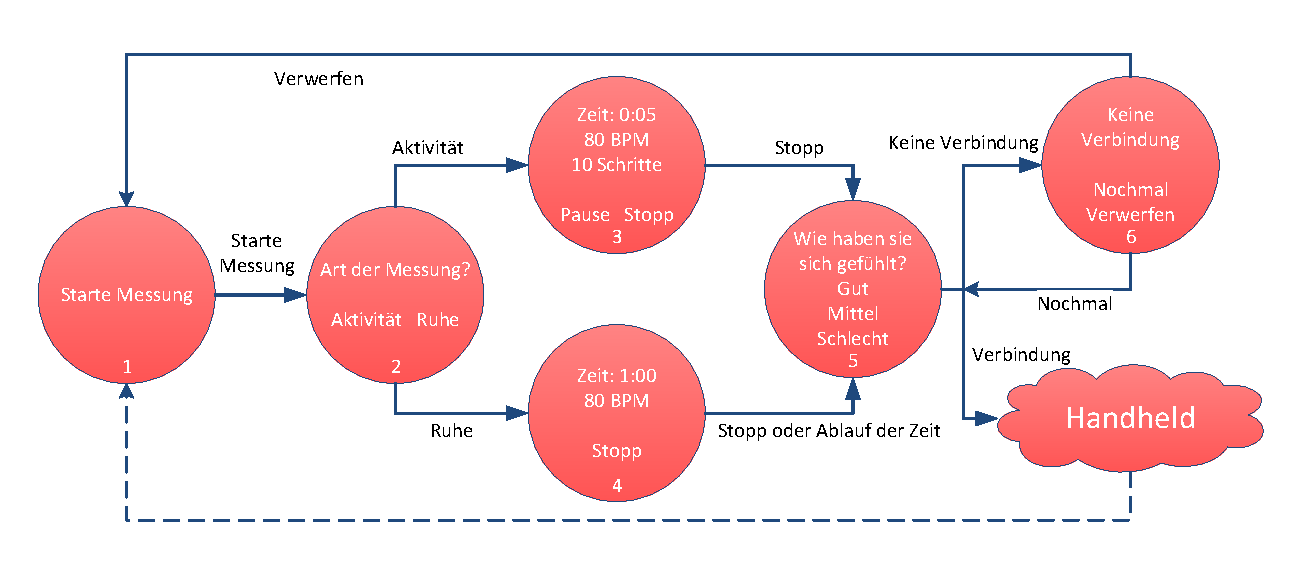
\includegraphics[scale=0.65]{images/structure_wearable.pdf}
	\caption{Struktur der Wearable-App}
	\label{fig:structure_wearable}
\end{figure}
\bigskip

Das Handheld-Gerät soll sich kontinuierlich in Bereitschaft zum Empfang von Messdaten befinden und diese verarbeiten können. Zusätzlich soll die App auf dem Handheld-Gerät über eine grafische Oberfläche zur Konfiguration und zur temporären Verwaltung von Messdaten verfügen. Ein Graph soll die Messungen übersichtlich visualisieren. Eine Bewertung der Daten ist an dieser Stelle nicht erforderlich.
\\[0.5cm] 
Das Handheld-Gerät soll die Messdaten per Bluetooth an ein Bluetooth-fähiges Endgerät weiter versenden können (z.B. PC oder Notebook). Es soll sowohl möglich sein, die Daten automatisch durch den Hintergrund-Dienst versenden zu lassen, als auch die Daten manuell über die grafische Oberfläche zu versenden. Die geplante Struktur der Handheld-App wird in Abbildung \ref{fig:strucure_handheld} dargestellt.

\bigskip
\begin{figure}[H]
	\visioToPDF{images/strucure_handheld.vsd}
	\centering
	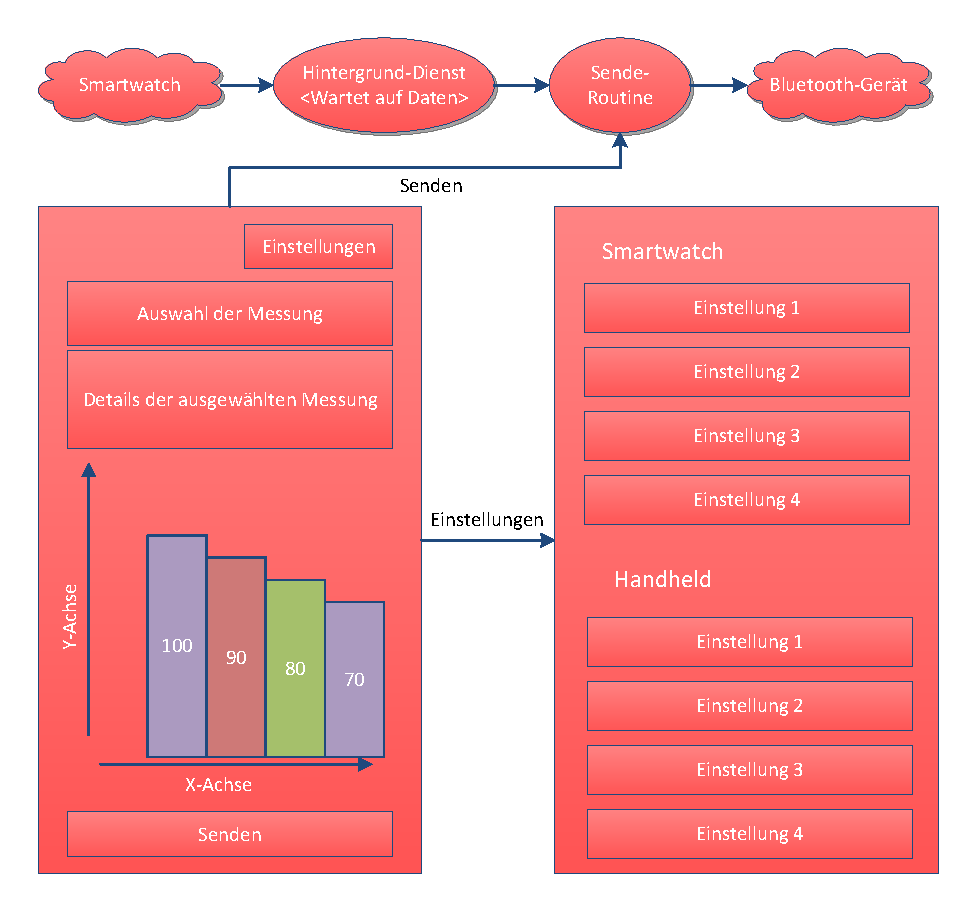
\includegraphics[scale=0.65]{images/strucure_handheld.pdf}
	\caption{Struktur der Handheld-App}
	\label{fig:strucure_handheld}
\end{figure}
\bigskip

\subsection{Vorbereitung}
Im Rahmen des Projektes werden eine Motorola Moto 360 Smartwatch und ein Samsung Galaxy S4 Smartphone als Testgeräte verwendet. Auf der Moto 360 läuft Android Wear in der Version 5.0 und auf dem Galaxy S4 läuft Android in der Version 4.4 (Cyanogenmod 11 Custom-Rom). Die Geräte sind grundsätzlich gekoppelt und die gleichnamige Google App "`Android Wear"' verwaltet auf dem Smartphone (im Hintergrund) die Verbindung zur Smartwatch. Die Entwicklung erfolgt mit Hilfe der Entwicklungsumgebung "`Android Studio"', die ebenfalls von Google veröffentlicht wurde. Dabei kann die Smartphone-App direkt über USB "`debugged"' werden, während der Debugging-Vorgang bei der Smartwatch über das gekoppelte Smartphone per Bluetooth gebrückt wird.

\subsection{Einschränkungen}
Bei Verwendung der Bluetooth-Library in der Qt-Framework Anwendung konnten Inkompatibilitäten nicht umgegangen werden (Näheres im Abschnitt QT Framework Anwendung). Aus diesem Grund soll die von der Handheld-App ausgehende Verbindung als TCP/IP Verbindung implementiert werden. Dabei soll ein UDP-Broadcast verwendet werden, um die Handheld-App im Netzwerk bekannt zu machen. Alternativ kann aber auch eine feste Adressierung angegeben werden. Da das Software-Paket sich letztlich an den gewöhnlichen Heimanwender richtet, ist grundsätzlich ein Heimnetzwerk mit Router und verbundenen Endgeräten zu erwarten und diese Anpassung sogar der Bluetooth-Variante vorzuziehen, da Bluetooth-Hardware zwar an Notebooks, jedoch vergleichsweise selten an feststehenden PCs verfügbar ist.

\subsection{Implementierung}
Die Implementierung teilt sich in drei Unterabschnitte zur Beschreibung: Die gemeinsame Bibliothek, die Wearable-App und die Handheld-App.
\subsubsection{Common-Library}
Die beiden Apps für das Wearable- und das Handheld-Gerät teilen sich eine Bibliothek um gemeinsame Datenstrukturen einfacher zu organisieren. \textit{HeartRateData} bildet einen Datensatz einer Messung ab, während \textit{HeartRateMeasure} eine umfassende Messung inklusive Modus, Stimmung und Durchschnittswert repräsentiert. Hier finden sich zusätzlich Methoden zur Übertragung und Konvertierung der Daten. So werden die Messdaten über die Android Wearable-Message-API als String im CSV-Format gesendet. Die statische Klasse \textit{HeartRateFile} bietet Methoden zum Laden und persistenten Speichern der genannten Datenstrukturen an. Diese Methoden werden nur auf dem Handheld-Gerät verwendet, jedoch könnte das Wearable-Gerät in einer möglichen Erweiterung auch eine persistente Speicherung der Daten vornehmen. In \textit{ByteCodes} werden Prefix-Byte-Codes für die serielle Übertragung per TCP angegeben. Der Empfänger der Daten muss dabei ebenfalls diese Byte-Codes kennen. In Abbildung \ref{fig:classes_common} werden diese Klassen dargestellt. Zusätzlich werden innerhalb der Common-Library alle verwendeten Grafiken zentral angelegt, um Redundanzen zu vermeiden.

\bigskip
\begin{figure}[H]
	\centering
	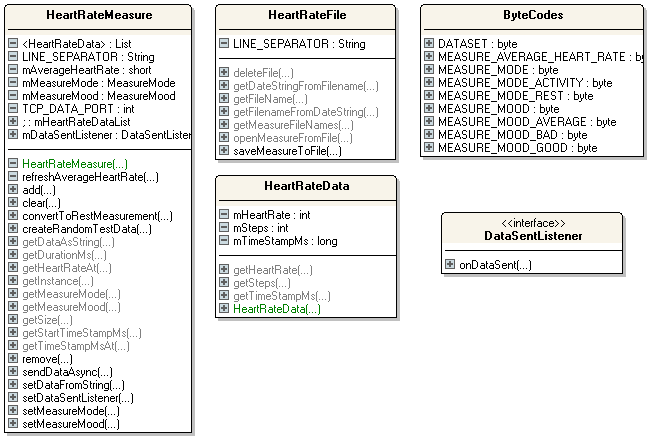
\includegraphics[scale=0.75]{images/classes_common.png}
	\caption{Klassendiagramm: Common-Library}
	\label{fig:classes_common}
\end{figure}
\bigskip

\subsubsection{Wearable-App}
Die Wearable-App teilt sich in verschiedene Grundkomponenten. Dabei bildet die Klasse \textit{WearActivity} das Zentrum der Ausführung. Sie wird von der Android-Klasse \textit{Activity} abgeleitet und dazu verwendet um eine Programmlogik mit Layout-Inhalten zu verknüpfen. Das WearActivity-Layout (siehe Abbildung \ref{fig:layout_wearactivity}) enthält alle grafischen Elemente, die zur Funktionalität benötigt werden:\\
\begin{minipage}[c]{0.5\textwidth}
	\begin{itemize}
		\item Zeitzähler inkl. Symbol
		\item Schrittzähler inkl. Symbol
		\item Puls
		\item Startbutton / Pausebutton
		\item Stoppbutton
		\item Hintergrundanimation
	\end{itemize}
\end{minipage}
\begin{minipage}[c]{0.5\textwidth}
	\begin{figure}[H]
		\centering
		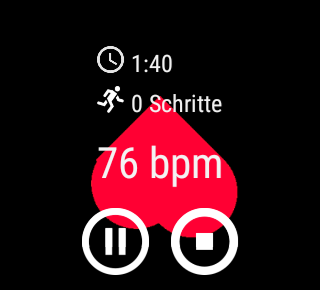
\includegraphics[scale=0.55]{images/layout_wearactivity.png}
		\caption{Layout: WearActivity}
		\label{fig:layout_wearactivity}
	\end{figure}
\end{minipage}
\\[0.7cm]
Die Hintergrundanimation (ein animiertes Herz-Symbol) besteht aus 32 Einzelbildern, die per XML-Animationsdatei aufeinander folgend abgespielt werden. Die Programmlogik der Hauptklasse \textit{WearActivity} basiert auf einem Zustandsautomaten. Elemente, die im jeweiligen Zustand nicht benötigt werden, werden ausgeblendet und umgekehrt. Analog zur Nummerierung in Abbildung \ref{fig:structure_wearable} finden sich die Zustände hier wieder. Die Zustände 2, 5 und 6 zur manuellen Abfrage von Informationen werden allerdings in externe Dialoge ausgelagert, da das Layout sich dort grundlegend ändert.
\\[0.5cm]
Diese Dialoge werden wiederum durch eigene Activitys repräsentiert und von der \textit{WearActivity} mittels Aufruf der Methode \textit{startActivity} gestartet. Sie liefern bei Beendigung einen entsprechenden Return-Wert. Abbildung \ref{fig:layout_dialogs} zeigt das Layout der drei Dialoge.
\bigskip
\begin{figure}[H]
	\centering
	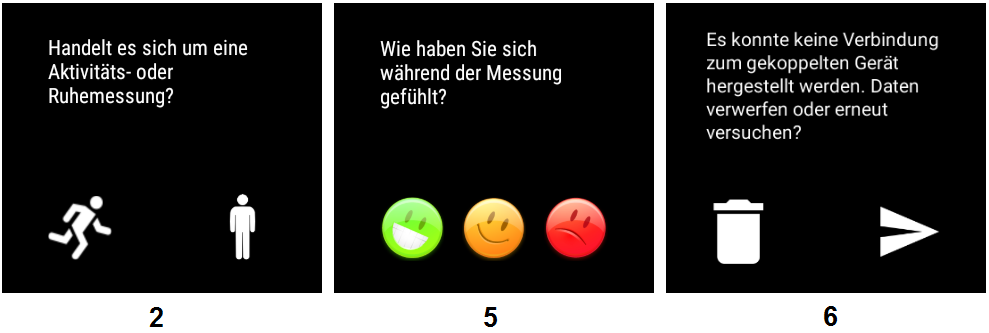
\includegraphics[scale=0.53]{images/layout_dialogs.png}
	\caption{Layout: Dialoge}
	\label{fig:layout_dialogs}
\end{figure}
\bigskip
Bei der Gestaltung der Wearable-Layouts wird das \textit{BoxInsetLayout} als Container verwendet, um eine äquivalente Darstellung auf quadratischen und runden Geräten zu erzielen und nur ein Layout für beide Display-Typen bereitstellen zu müssen. 
\\[0.5cm]
Abgesehen von den Activity-Klassen gibt es noch andere Klassen, die an der Umsetzung der Programmlogik innerhalb der Wearable-App beteiligt sind. So gibt es beispielsweise die Klasse \textit{RunningTimer}, die den Timer für Aktivitätsmessungen implementiert. Dabei kann eine beliebige Zeitspanne zum Auslösen des Events \textit{onTimerUpdate} angegeben werden. Das Event wird innerhalb der \textit{WearActivity}-Klasse genutzt um die Timer-Information auf der grafischen Oberfläche zu aktualisieren. Mit dem Event verbunden ist auch die regelmäßige Erinnerung (Vibrationsmuster bzw. Meldung), dass die App noch aktiv ist.
\\[0.5cm]
Daneben gibt es noch die Klasse \textit{RestTimer}, die die Ruhemessung unterstützt. Hier wird eine festgelegte Zeitspanne rückwärts gezählt und im Anschluss das Event \textit{onTimerFinished} ausgelöst. Analog zur Klasse \textit{RunningTimer} gibt es ebenfalls ein Event \textit{onTimerUpdate} zur Aktualisierung der Oberfläche.
\\[0.5cm]
Die wichtigste Komponente zur Erfassung der Sensor-Daten ist die Klasse \textit{SensorLogger}, die den Zugriff auf den Puls- und Schrittsensor verwaltet. Innerhalb des internen Events \textit{onSensorChanged} werden für beide Sensoren die entsprechenden Werte gespeichert und ein neues Event \textit{onSensorLog} zur Verwendung in der \textit{WearActivity}-Klasse abstrahiert. \textit{SensorLogger} bietet Methoden zum Starten, Stoppen und Pausieren des Logging-Vorgangs an. Auch das Messungsintervall kann festgelegt werden.
\\[0.5cm]
Eine weitere wichtige Komponente ist die Singleton-Klasse \textit{HeartRateDataSync}, die mit Hilfe der Wearable-Message-API einen String zu allen verbundenen Handheld-Geräten überträgt. Durch die Pfad-Angabe ("`/heartrate2go-message"') kann der Listener-Service am anderen Ende die App der Nachricht zuordnen.
\\[0.5cm]
Den letzten Bestandteil der Wearable-App bilden die Klassen \textit{DataLayerListenerService} und \textit{Settings}. Die Klasse \textit{DataLayerListenerService} wird von der Android-Klasse \textit{WearableListenerService} abgeleitet, die zur Verarbeitung eingehender Kommunikation seitens Wearable-API verwendet wird. Eine gleichnamige Klasse wird auf dem Handheld-Gerät ebenfalls verwendet, um die von \textit{HeartRateDataSync} ausgehenden Nachrichten zu empfangen. Auf dem Wearable-Gerät wird die Implementierung dieser Struktur lediglich für den Empfang von Settings-Werten benötigt. Dabei werden die Einstellungen innerhalb einer Hash-Map übertragen, da die Einstellungen selbst auch als Key-Value-Paare vorliegen. Die Klasse \textit{Settings} wird verwendet, um Zugriff auf die Klasse \textit{SharedPreferences} und die enthalten Einstellungen zu abstrahieren.
\\[0.5cm]
Die Zusammenhänge werden im Klassendiagramm der Abbildung \ref{fig:classes_wearable} noch einmal verdeutlicht.
\bigskip
\begin{figure}[H]
	\centering
	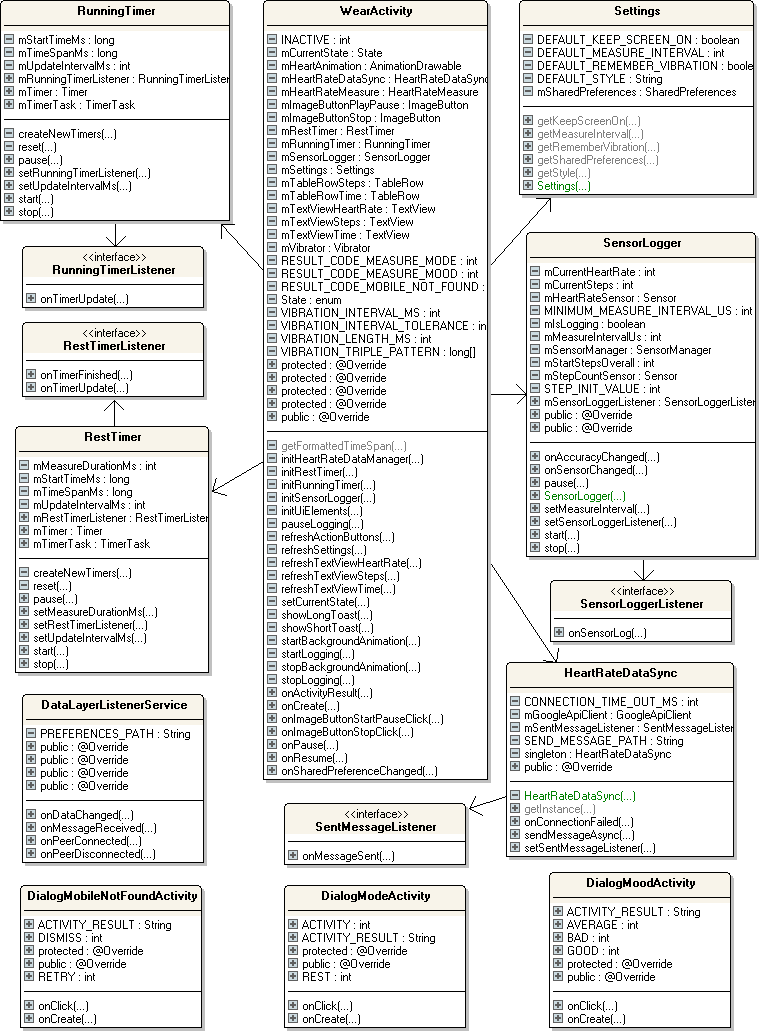
\includegraphics[scale=0.7]{images/classes_wearable.png}
	\caption{Klassendiagramm: Wearable-App}
	\label{fig:classes_wearable}
\end{figure}
\bigskip

\subsubsection{Handheld-App}
Die Handheld-App dient primär zur Weiterübertragung der über Bluetooth empfangenen Mess-Daten an eine externe Anwendung über TCP. Daneben werden auch Daten grafisch als Diagramm dargestellt und persistent vorrätig gehalten. Zur Diagramm-Darstellung wird sich der freien Library \textit{GraphView}\cite{graphview} bedient. Über eine Drop-Down-Liste kann eine Messung zur Anzeige ausgewählt werden. Eine ausgewählte Messung kann manuell über TCP versendet werden, gelöscht werden oder Beides gleichzeitig. Der Settings-Dialog der Handheld-App lässt verschiedene Einstellungen für Handheld-App und Wearable-App vornehmen, wie Abbildung \ref{fig:layout_settings} zeigt. Abbildung \ref{fig:classes_handheld} zeigt ein Klassendiagramm der Handheld-App.\\

\begin{minipage}[c]{0.5\textwidth}
	\begin{figure}[H]
		\centering
		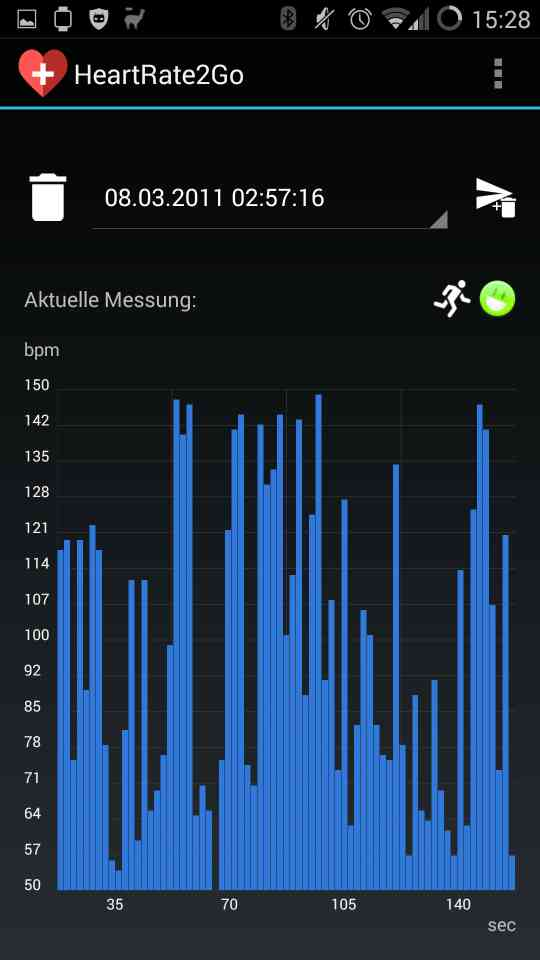
\includegraphics[scale=0.3]{images/layout_handheld.jpg}
		\caption{Layout: Handheld}
		\label{fig:layout_handheld}
	\end{figure}
\end{minipage}
\begin{minipage}[c]{0.5\textwidth}
	\begin{figure}[H]
		\centering
		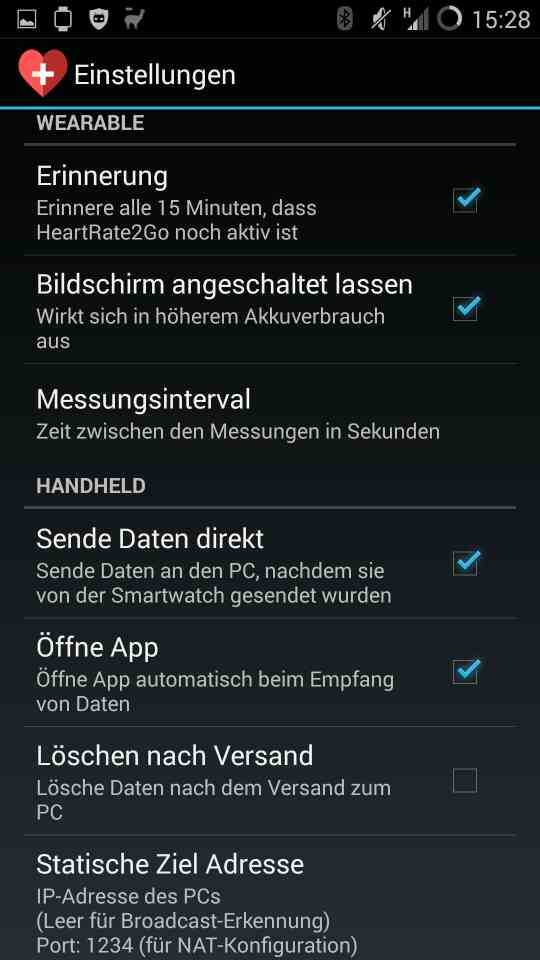
\includegraphics[scale=0.3]{images/layout_settings.jpg}
		\caption{Layout: Settings}
		\label{fig:layout_settings}
	\end{figure}
\end{minipage}
\\[0.7cm]

Die Handheld-App verfügt neben der Settings-Activity über eine Haupt-Activity \textit{HandheldActivity} zur Darstellung der Oberflächeninhalte. Die beschriebenen, überschaubaren Funktionen sind hier zentral verfügbar. Abbildung \ref{fig:layout_handheld} zeigt das zugehörige Layout.
\\[0.5cm]
Der Vorgang zum Senden der Messdaten über TCP ist innerhalb der Common-Klasse \textit{HeartRateMeasure} als Methode zu finden. Als Parameter muss lediglich die IP-Adresse übergeben werden. Innerhalb dieser Methode werden die Objektdaten mit Hilfe der Prefix-Byte-Codes serialisiert und als Byte-Stream versendet. Im Anschluss an den Sende-Vorgang berichtet das Event \textit{onDataSent} über den Status.
\\[0.5cm]
Die Klasse \textit{NetworkBroadcast} dient zur einfachen Identifizierung vor TCP-Gegenstellen im Netzwerk. Hierfür wird ein Magic-Packet per UDP-Broadcast in das lokale Netz gesendet und das Event \textit{onBroadcastFinished} ausgelöst, das bei Erfolg die IP-Adresse des Empfängers und dessen Antwort übergibt. Die Verwendung des Broadcasts ist einstellungsabhängig. Die Angabe einer statischen IP-Adresse ist ebenfalls möglich, womit der Broadcast umgangen wird.
\\[0.5cm]
Letztlich ist die Klasse \textit{DataLayerListenerService} für den Empfang der Messdaten von der Wearable-App verantwortlich und bildet das zentrale Element der Handheld-App. Bei eingehenden Messdaten wird der Service gestartet und sendet - je nach Einstellung - die Daten im Hintergrund unmittelbar zur TCP-Gegenstelle weiter. Entsprechend wird, bei aktivierter Einstellung zum Starten der App, die Oberflächen-Activity beim Empfangen von Daten mit gestartet und zeigt die aktuelle Messung an.
\\[0.5cm]


\bigskip
\begin{figure}[H]
	\centering
	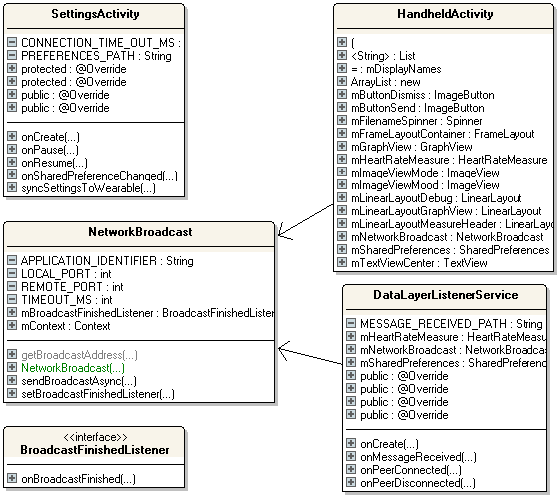
\includegraphics[scale=0.7]{images/classes_handheld.png}
	\caption{Klassendiagramm: Handheld-App}
	\label{fig:classes_handheld}
\end{figure}
\bigskip

\subsection{Evaluierung}
Es werden unterschiedliche Testfälle hinsichtlich Fehlerverhalten bei den vorgesehenen Ausführungsroutinen angefertigt und geprüft. Die Testfälle und deren Ergebnisse werden tabellarisch aufgelistet.
\subsubsection{Wearable-App}
Im Vordergrund steht bei der Wearable-App die ständige Definiertheit des Zustandsautomaten. In folgender Tabelle \ref{tbl:testcases_wearable} werden alle Zustände, Zustandsänderungen und Folgezustände aufgelistet und verifiziert. Die in Abbildung \ref{fig:structure_wearable} gezeigte Zustandsabfolge gilt hier als Referenz.

\begin{table*}[h]
	\centering
	  \rowcolors{1}{}{lightgray}
		\begin{tabularx}{\textwidth}{lXlc}
			\textbf{Zustand} 			& \textbf{Änderung} 	& \textbf{Folgezustand} 	&  \\
			Start (1) 						& Starte Messung 			& Messungsabfrage (2) 		& \ok \\
			Messungsabfrage (2) 	& Aktivität 					& Aktivitätsmessung (3) 	& \ok \\
			Aktivitätsmessung (3) & Pause 							& Aktivitätsmessung (3) 	& \ok \\
			Aktivitätsmessung (3) & Stopp 							& Stimmungsabfrage (5) 		& \ok \\
			Messungsabfrage (2) 	& Ruhe 								& Ruhemessung (4) 				& \ok \\
			Ruhemessung (4) 			& Stopp 							& Stimmungsabfrage (5) 		& \ok \\
			Stimmungsabfrage (5) 	& + Verbindung 				& Start (1) 							& \ok \\
			Stimmungsabfrage (5) 	& - Verbindung 				& Retry-Abfrage (6) 			& \ok \\
			Retry-Abfrage (6) 		& Retry + Verbindung 	& Start (1) 							& \ok \\
			Retry-Abfrage (6) 		& Retry - Verbindung 	& Retry-Abfrage (6) 			& \ok \\
		\end{tabularx}
		\caption{Testfälle: Wearable}
		\label{tbl:testcases_wearable}
\end{table*}

\subsubsection{Handheld-App}
Die Handheld-App muss in der Rolle des Daten-Vermittlers zwischen Wearable-Gerät und IP-Endgerät die Messdaten zuverlässig und unverändert weiterleiten. Die korrekte Darstellung von Messdaten ist ebenfalls ein Testkriterium. Außerdem wird die Anwendung und Übertragung von Einstellungen geprüft. Die nachstehende Tabellen \ref{tbl:testcases_handheld_behavior} und \ref{tbl:testcases_handheld_settings} zeigen die Testkriterien auf.

\begin{table*}[h]
	\centering
	  \rowcolors{1}{}{lightgray}
		\begin{tabularx}{\linewidth}{Xc}
			\textbf{Testfall}																		& \\
			Daten auf grafischer Oberfläche korrekt anzeigen		& \ok \\
			Daten mit Hintergrund-Dienst versenden							& \ok \\
			Daten mit grafischer Oberfläche versenden						& \ok \\
			Toast über Versende-Status anzeigen									& \ok \\
			Daten löschen			 																	& \ok \\
			Zufällige Daten erzeugen (Debugmodus)								& \ok \\
			Alle Datensätze versenden (Debugmodus)							& \ok \\
			Daten bei nur bei erfolgreicher Verbindung löschen	& \ok \\
		\end{tabularx}
		\caption{Testfälle: Handheld-Verhalten}
		\label{tbl:testcases_handheld_behavior}
\end{table*}

\begin{table*}[h]
	\centering
	  \rowcolors{1}{}{lightgray}
		\begin{tabularx}{\linewidth}{Xlc}
			\textbf{Einstellung}						& \textbf{Typ} 				& \\
			Erinnerung											& Wearable 						& \ok \\
			Bildschirm angeschaltet lassen 	& Wearable 						& \ok \\
			Messungsintervall 							& Wearable 						& \ok \\
			Sende Daten direkt 							& Handheld 						& \ok \\
			Öffne App automatisch						& Handheld 						& \ok \\
			Löschen nach Versand						& Handheld 						& \ok \\
			Statische Ziel-Adresse					& Handheld 						& \ok \\
			Debug-Modus							 				& Handheld 						& \ok \\
		\end{tabularx}
		\caption{Testfälle: Handheld-Einstellungen}
		\label{tbl:testcases_handheld_settings}
\end{table*}

%\lstset{language=Java}
%\begin{lstlisting}[caption=Listing, label=lst:Listing]
%\end{lstlisting}

%\begin{shaded}
%Text in Textbox
%\end{shaded}

%\ref{sec:hauptteil}
%\cite{audio_architecture}